\documentclass{boi2014-lt}

\usepackage{enumitem}
\usepackage{todonotes}
\usepackage{wrapfig}

\renewcommand{\DayNum}{2}
\renewcommand{\TaskCode}{demarcation}
\renewcommand{\TaskName}{Demarkacija}

\newcommand{\constant}[1]{{\tt #1}}

\begin{document}
    \begin{wrapfigure}{r}{3cm}
        \vspace{-24pt}
		\includegraphics[width=3cm]{\TaskCode.jpeg}
	\end{wrapfigure}

    Karalius Baitazaras ilgai ir teisingai valdė Baitopijos salą. Tačiau po
    staigios mirties jo sūnūs dvyniai --- Baitonas ir Bitonas --- niekaip
    negalėjo sutarti, kuris iš jų turėtų paveldėti sostą. Jie nusprendė
    padalinti salą į dvi provincijas, kad galėtų jas valdyti nepriklausomai.
 
    Stačiakampyje žemėlapyje Baitopija yra $N$ kraštinių turintis daugiakampis.
    Visos daugiakampio kraštinės yra lygiagrečios žemėlapio kraštinėms, o
    kiekviena gretima daugiakampio kraštinė yra statmena viena kitai. Jokia
    daugiakampio kraštinė nekerta ir neliečia jokios kitos kraštinės, išskyrus
    gretimų kraštinių galus.

    Baitonas ir Bitonas norėtų padalinti salą į du kongruenčius daugiakampius
    viena atkarpa, kuri būtų salos daugiakampio viduje ir būtų lygiagreti
    žemėlapio kraštinei. (Du daugiakampiai yra kongruentūs jeigu vienas iš jų
    gali būti transformuotas į kitą kokia nors atspindžio, posūkio arba poslinkio
    operacijų kombinacija.) Visų daugiakampio viršūnių ir ieškomos dalinančios
    atkarpos galų koordinatės yra sveikieji skaičiai.
 
    Karaliaus sūnūs prašo jūsų patikrinti, ar toks salos padalinimas yra
    įmanomas.

    \Task
    Duotai salos formai nustatykite, ar ji gali būti padalinta horizontalia arba
    vertikalia atkarpa į du kongruenčius daugiakampius. Jeigu toks padalinimas
    egzistuoja, raskite salą dalinančią atkarpą.

    \Input
    Pirmoje eilutėje įrašytas vienas sveikasis skaičius $N$ -- daugiakampio
    viršūnių skaičius. Toliau $i$-ojoje iš $N$ eilučių įrašyta tarpais atskirta
    sveikųjų skaičių pora $X_i$ ir $Y_i$ ($0 \le X_i, Y_i \le 10^9$) -- $i$-osios
    viršūnės koordinatės.
    
    Viršūnės pateiktos tokia tvarka, kad atkarpos $(X_1,Y_1) - (X_2,Y_2)$,
    $(X_2,Y_2) - (X_3,Y_3)$, \ldots, $(X_{N-1},Y_{N-1}) - (X_N,Y_N)$ ir
    $(X_N,Y_N) - (X_1,Y_1)$ yra visos daugiakampio kraštinės. Be to, bet kurios
    dvi iš eilės einančios atkarpos yra viena kitai statmenos.

    \Output
    Jūsų programa turėtų išvesti vieną eilutę. Jeigu įmanoma padalinti salą į du
    kongruenčius daugiakampius horizontalia arba vertikalia atkarpa, kurios galų
    koordinatės yra $(x_1, y_1)$ ir $(x_2, y_2)$, išspausdinkite $4$ tarpais
    atskirtus sveikuosius skaičius $x_1$, $y_1$, $x_2$ ir $y_2$. Jiems turėtų
    galioti bent viena iš lygybių $x_1 = x_2$ arba $y_1 = y_2$. Ši atkarpa
    turėtų būti daugiakampio viduje ir tik jos galai turėtų liesti daugiakampio
    ribą.

    Jeigu neįmanoma rasti tinkamo salos padalinimo, išveskite vieną žodį
    \constant{NO}.
    
    \pagebreak

    \Examples
	\example
	{
		10 \newline
		0 0 \newline
		1 0 \newline
		1 1 \newline
		3 1 \newline
		3 5 \newline
		2 5 \newline
		2 3 \newline
		1 3 \newline
		1 2 \newline
		0 2
	}
	{
		1 2 3 2
	}
	{
		Atkreipkite dėmesį, kad $3 2 1 2$ irgi yra teisingas atsakymas.
		
        \begin{center}
            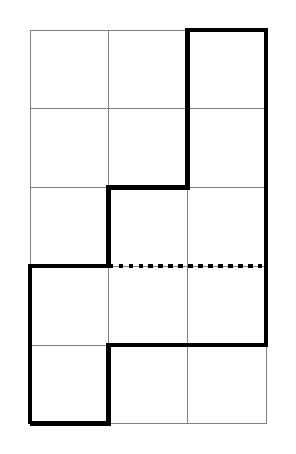
\begin{tikzpicture}
            \draw[help lines] (0,0) grid (3,5);
            \draw[ultra thick] (0,0) -- (1,0) -- (1,1) -- (3,1) -- (3,5) --
                         (2,5) -- (2,3) -- (1,3) -- (1,2) -- (0,2) -- (0,0);
            \draw[ultra thick,dotted] (1,2) -- (3,2);
            \end{tikzpicture}
        \end{center}
	}

	\example
	{
		6 \newline
		0 0 \newline
		1 0 \newline
		1 1 \newline
		2 1 \newline
		2 2 \newline
		0 2
	}
	{
		NO
	}
	{
        Šiuo atveju padalinti salą į du kongruenčius daugiakampius yra neįmanoma.
        \begin{center}
            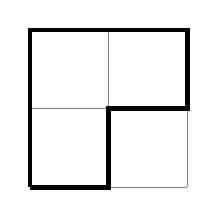
\begin{tikzpicture}
            \draw[help lines] (0,0) grid (2,2);
            \draw[ultra thick] (0,0) -- (1,0) -- (1,1) --
                         (2,1) -- (2,2) -- (0,2) -- (0,0);
            \end{tikzpicture}
        \end{center}
	}

    \Scoring

    \begin{description}
        \item[Dalinė užduotis nr. 1 (? taškų).] $4 \le N \le 100\ 000$.
            Bet kuri horizontali arba vertikali tiesė, kuri kerta daugiakampį,
            dalina daugiakampį į lygiai dvi dalis.
        \item[Dalinė užduotis nr. 2 (? taškų).] $4 \le N \le 200$
        \item[Dalinė užduotis nr. 3 (? taškų).] $4 \le N \le 4\ 000$
        \item[Dalinė užduotis nr. 4 (? taškų).] $4 \le N \le 100\ 000$
    \end{description}

    \Constraints

    \begin{description}
        \item[Laiko limitas:] 0,5 s.
        \item[Atminties limitas:] 256 MB.
    \end{description}

\end{document}
